\chapter{Data and Methods}
\label{ch:methods}

In this thesis, several different observational and reanalysis data sets, as well as model simulations, are used. For example, the reanalysis data sets are employed in \chapref{ch:simple_cld_scheme} to derive the linear formula between cloud fraction and relative humidity, and to evaluate the relationship between low cloud amount and its possible proxies. The satellite products about clouds and radiation fields are used in \chapref{ch:eval_cld_scheme} to evaluate the performance of the simple cloud scheme. To make it clear, these data sets are briefly summarized in this chapter.

The major topic of this thesis is about the cloud feedback, and the main tool used to simulate it is the idealized climate model, Isca \citep{Vallis2018}. Therefore, the features of this climate model and the advantages of using the idealized models are discussed here. However, how to calculate or estimate cloud feedback in climate models is not so evident, and the direct estimate from the change of cloud radiative effect might be impacted by the cloud masking effect. Therefore, it is necessary to discuss the pros and cons of the several different methods to estimate cloud feedback in this chapter. Also, based on these discussion, it would be much easier for Isca to calculate the cloud feedback and decompose it into different components if the cloud simulator is implemented there, so the topic about this is also presented in this chapter. 

The chapter is organized as follows: The satellite data sets related to radiation and cloud fields are introduced in \secref{sec:obs_reanalysis_dataset}. The idealized general circulation model employed throughout this thesis is briefly described in \secref{sec:isca_intro}. In \secref{sec:cosp}, how the cloud observation simulator package is implemented in Isca is documented. \secref{sec:method_cloud_fbk} summarizes the possible methods to calculate the cloud feedback.

\section{Observational and reanalysis datasets}
\label{sec:obs_reanalysis_dataset}

\subsection{Satellite datasets}
Satellites play important roles in observing the Earth (not limit to clouds and radiation) over the past decades, and these satellite retrievals are essential data sets for us to understand the weather and climate on Earth. In general, the satellite products can be categorized into different groups according to their processing levels ranging from Level 0 to Level 4 \citep{Parkinson2006earth}. Specifically, Level 0 is the raw and unprocessed instrument data. Level 1 is annotated with ancillary information (1A) and processed to sensor units (1B). Level 2 is derived geophysical variables, Level 3 is mapped to a space-time grid, and Level 4 are modeled outputs or variables derived from multiple measurements. It is usually easier for users to use these satellite retrievals when they have higher processing levels. 

% (see \url{https://earthdata.nasa.gov/collaborate/open-data-services-and-software/data-information-policy/data-levels}, last accessed: April 28, 2021)
% https://nsidc.org/the-drift/2013/08/is-it-1b-2-or-3-definitions-of-data-processing-levels/

% \begin{itemize}
%     \item \textbf{Level 0}:	Reconstructed, unprocessed instrument and payload data at full resolution, with the communications artifacts removed.
%     \item \textbf{Level 1A}: The Level 0 data with time-reference and with ancillary information
%     \item \textbf{Level 1B}: Same as Level 1A data, but have been processed to sensor units (not all instruments have Level 1B source data)
%     \item \textbf{Level 2}:	Derived geophysical variables at the same resolution and location as Level 1 source data.
%     \item \textbf{Level 3}:	Variables mapped on uniform space-time grid scales, usually with some completeness and consistency.
%     \item \textbf{Level 4}:	Model output or variables derived from multiple measurements.
% \end{itemize}


\subsubsection{Clouds and the Earth’s Radiant Energy System  Top-of-Atmosphere (TOA) data product}
% Energy Balanced and Filled (EBAF)

The Clouds and the Earth’s Radiant Energy System (CERES) project (\url{https://ceres.larc.nasa.gov}) provides satellite-based observations of Earth's radiation budget and clouds. It uses measurements from CERES instruments flying on several satellites (TRMM\footnote{TRMM: Tropical Rainfall Measuring Mission, a research satellite in operation from 1997 to 2015}, Terra, Aqua, S-NPP\footnote{S-NPP: Suomi National Polar-orbiting Partnership}, NOAA-20\footnote{NOAA-20: National Oceanic and Atmospheric Administration-20}), along with measurements from higher-resolution imagers on polar orbiting and geostationary satellites and other input data source, to produce a comprehensive set of Earth's radiaiton budget data products for weather, climate and applied science research. The goal of CERES is to produce a long-term, integrated global climate data record for detecting decadal changes in the Earth’s radiation budget from the surface to the top of the atmosphere, so as to improve our understanding of how Earth’s radiation budget varies in time and space and of the role that clouds and other atmospheric properties play.


\subsubsection{International Satellite Cloud Climatology Project (ISCCP) -- H Series}

The International Satellite Cloud Climatology Project (ISCCP) began in early 1980s as part of the World Climate Research Program (WCRP) \citep{Schiffer1983,Rossow1991}, and is probably the longest-running international satellite-based global environmental data project. Its goal is to collect weather satellite radiance measurements and to analyze them to infer the global distribution of clouds, their properties, and their diurnal, seasonal and interannual variations. This project has accumulated cloud observation for almost four decades and has been therefore widely used in cloud related researches.

Several series of the ISCCP products hve been publised previously. However, the widely used ISCCP D-series product \citep{Rossow1999advances} has not been updated since December 2009. Recently, a new H-series product was published \citep{Young2018}, spanning from 1982 to 2015 (see \url{https://isccp.giss.nasa.gov/products/onlineData.html}, last accessed: April 28, 2021). Comparing to the previous ISCCP D-series product, the H-series has improved the low-level cloud sensitivity over snow and ice in polar regions. More importantly, based on ISCCP’s legacy and in light of the technological advancements that include active spaceborne sensors (e.g., Cloud–Aerosol Lidar and Infrared Pathfinder Satellite Observations – CALIPSO – and CloudSat) and cloud data sets that rely on newer passive imagers with higher spectral, spatial, radiometric, and temporal resolutions, the H-series has exploited to produce cloud products with much higher resolutions \citep{Young2018}.

In this study, the high-resolution global monthly (HGM) product (at Level 3) with $1^\circ \times 1^\circ$ resolution is used for analysis. Of course, gridded hourly high-resolution output (HGH) is also available. In ISCCP H-series product, it has provided many cloud related variables, such as (but are not limited to) cloud amount (low, middle, high and total), cloud-top temperature, cloud-top pressure, cloud optical thickness, cloud water path, cloud phase and cloud type.

\subsubsection{CloudSat Radar-Only Cloud Water Content (2B-CWC-RO) product}

The CloudSat Radar-Only Cloud Water Content (2B-CWC-RO) product contains retrievals of cloud liquid and ice water content, effective radius of the ice and liquid particles, number concentration, and the size distribution width parameter using radar and auxiliary temperature data \citep{Austin2009}. The latest release P1\_05 is used in this study. Retrievals are performed separately for the liquid and ice phases assuming liquid only and ice only, then the two sets combined in a simple way to obtain a composite profile that is consistent with the input measurements. The partition of ice and liquid is purely based on temperature, and the solutions of ice and liquid are scaled linearly with temperature to obtain a smooth transition from all ice at −20$^\circ$C to all liquid at 0$^\circ$C. The retrieval uses a temperature dependent a priori of lognormal (a modified gamma distribution) size distribution parameters, which are fitted from in situ particle size spectra.  
% Refer to: https://agupubs.onlinelibrary.wiley.com/doi/full/10.1029/2020EA001147

In this study, we choose to use the CloudSat 2B-CWC-RO product for cloud water path rather than the CERES-EBAF data set, because previous study has shown that CloudSat 2B-CWC-RO product can better represent cloud liquid and ice water path over high latitudes than CERES-EBAF data set, owing to its explicit determination of cloud phase \citep{Lenaerts2017}. But we should notice that CloudSat 2B-CWC-RO product also has some potential problems. For example, \cite{Barker2008} has shown the temperature-partitioned profiles could not capture the mixed phased cloud structure accurately.

%The cloud water path is from the CloudSat \index{CloudSat} 2B-CWC-RO Release P1\_R05 data product \citep{Austin2009} from 2012 to 2016, which can better represent cloud liquid and ice water path over high latitudes than CERES-EBAF data set, owing to its explicit determination of cloud phase \citep{Lenaerts2017}. The original CloudSat cloud water path data set has some missing data for certain dates, and is not in the T42 resolution we are going to use. To get the annual mean product we desired, the original data set is processed as follows: For the area each grid point covers, the total times that the satellite has visited over the 5 years and the sum of the cloud water path that has been retrieved over same period are recorded, from which the annual mean cloud water path is derived. The scripts to do this can be accessed at \url{https://github.com/lqxyz/cloudsat_cloud_water_path}.


\subsection{Reanalysis data sets}

\subsubsection{European Centre for Medium-Range Weather Forecasting (ECMWF) Interim Reanalysis (ERA-Interim)}

\section{Isca}
\label{sec:isca_intro}
\subsection{Overview}
%\subsection{}

%\section{Climate feedback}

\section{CFMIP observation simulator pacakage}
\label{sec:cosp}

\section{The calculation of cloud feedback}
\label{sec:method_cloud_fbk}

\subsection{Introduction}

As introdued in \chapref{ch:literature_review_about_clouds}, 
the concept of climate feedback is used to characterize the response of climate system to external radiative forcing. If we assume the climate system is at equilibrium state, and when an external foring $\Delta Q$ is imposed to the climate system, which can be aroused from the perturbation of CO$_2$ concentration, change in solar constant, or volcanic eruption, the climate system will response to this radiative imbalance at the top of the atmosphere (TOA) by changing the surface temperature ($T_s$). Let $R$ be the radiation budget at TOA, and the radiation imbalance ($\Delta R$) goes to zero during the climate system adjusts towards a new equilibrium. Using the idea of feedback, $\Delta R$ can be linked to the change of surface temperature ($\Delta T_s$) as follows:
\begin{equation}
    \Delta R = \Delta Q + \lambda \Delta T_s,
    \label{eq:imbalance_forcing_lambda}
\end{equation}
in which $\lambda$ is called climate feedback parameter. Besides surface temperature, other variables such as atmospheric temperature, water vapor, albedo and cloud properties may also change, and thus might have an impact on $\lambda$ as well. In theory, the climate feedback parameter $\lambda$ can be evaluated as follows
\begin{equation}
    \lambda = \frac{\partial R}{\partial T_s} = \sum_x \frac{\partial R}{\partial x}\frac{\partial x}{\partial T_s}  + Re, %\text{high-order terms},
    %+  \sum_x\sum_y \frac{\partial^2 R}{\partial x\partial y}\frac{\partial x\partial y}{\partial^2 T_s}+\dots 
    \label{eq:lambda}
\end{equation}
where $x$ represent the climate variable such as temperature, water vapor, albedo and cloud properties. The high-order residual term ($Re$) is usually neglected in analysis.

\subsection{Short summary of three approaches}
\label{sec:three_climate_fbk_methods}

Several different methods have been proposed to diagnose climate feedbacks in gerenal ciculation models (GCMs). Three main approaches are summarized below. Readers may refer to Appendix B of \cite{Bony2006} for a clear summary of the first two methods.% and refer to several pioneering papers from Soden, Held and others for a detailed description of the third method  \citep[e.g.,][]{Soden2006,Soden2008,Shell2008}.

\begin{enumerate}[label={(\arabic*)}]
    \item \textbf{The PRP approach}\\
    The partial radiative perturbation (PRP) method \citep{Wetherald1988cloud} evaluates partial derivatives of model TOA radiation with respect to changes in model parameters by re-running the model radiation code offline. For example, to calculate the climate feedback parameter associated with $x$, the radiative response that results from the perturbation of $x$ is calculated as follows:
    %substituting one variable at a time from the perturbed climate state into the control climate.
    \begin{equation}
        \delta_x R = R(a,b,...,x') - R(a,b,...,x),
        \label{eq:delta_R_x}
    \end{equation}
    where $a$, $b$ etc are climate variables except $x$ and they are kept unchanged during calculation. $x'$ is the value of $x$ from perturbed climate state. In doing so, $\frac{\partial R}{\partial x}$ in \eqref{eq:lambda} can be obtained from this offline calculation. The feedback parameter associated with $x$ is finally computed from $\lambda_x = \frac{\partial R}{\partial x}\frac{\mathrm{d} x}{\mathrm{d} T_s}$, and $\frac{\mathrm{d} x}{\mathrm{d} T_s}$ is calculated by differencing the simulation outputs from two experiments or from different time periods. Note that a more accurate two-sided PRP method \citep{Colman1997} is also used to estimate the partial radiative responses at TOA, so \eqref{eq:delta_R_x} can be rewritten as
    \begin{equation}
        \delta_x R = \frac{1}{2} \left[R(a,b,...,x') - R(a,b,...,x) + R(a',b',...,x') - R(a',b',...,x) \right].
    \end{equation}
    The advantage of PRP method is that it can separate different climate feedbacks, including ones related to clouds. But the procedure can be computationally expensive \citep{Soden2008}, and the calculation  must be repeated for every simulation and climate model versions.
    % The parameters  from control and perturbed climate states are substituted one by one into radiation code to obtain the partial responses at TOA.
    
    \item \textbf{The CRE approach}\\
    The `cloud radiative effect' (CRE) approach \citep[or CRF in][]{Cess1990intercomparison, Cess1996cloud} decompose the climate feedback into clear-sky and cloudy components. They do so by decompose the total TOA radiation budget $R$ as the sum clear-sky component ($R_{clear}$) and CRE ($\mathrm{CRE}=R-R_{clear}$), so \eqref{eq:imbalance_forcing_lambda} can be written as
    \begin{equation}
        \lambda = \frac{\Delta R - \Delta Q}{\Delta T_s} = \underbrace{\frac{\Delta R_{clear} - \Delta Q}{\Delta T_s}}_{\text{clear-sky climate feedback}} + \underbrace{\frac{\Delta\mathrm{CRE}}{\Delta T_s}}_{\text{cloud feedback}}.
        \label{eq:CRE_approach}
    \end{equation}
    It is clear that this method can not separate the clear-sky climate feedback components into temperature, water vapor and surface albedo ones in further. As we will discuss in \secref{sec:CRE_or_PRP}, the cloud feedback parameter (second term in \eqref{eq:CRE_approach}) obtained from this approach depends on changes in both clear-sky and cloudy properties, which in fact can not separate the cloud feedback completely from the clear-sky components. Nevertheless, the calculation of this method is straightforward and still valuable in GCM evaluations.
    
    \item \textbf{The radiative kernel method}\\
    The radiative kernel method \citep[e.g.,][]{Soden2006,Soden2008,Shell2008} decompose each climate feedback into two parts. The first is the `radiative kernel' ($\partial R/\partial x$), which describes the change of TOA fluxes in response to a standard change in property $x$ and depends on the radiative properties and base state of the model. The second term is the climate response of feedback varaible normalized by surface temperature change ($\mathrm{d} x/\mathrm{d} T_s$). Most importantly, \cite{Soden2008} has shown the climate feedbacks calculated from three different radiative kernels are quite similar, although the radiative transfer code is different, indicating that a single kernel can be used to perform a first-order comparison of feedbacks across mutliple models \citep{Shell2008}. One problem is that the kernel calculation is also computationally expensive as it requres running the offline radiative transfer code for perturbation at each model level and time step, but luckily it just needs one-time calculation and the kernel can be applied for different experiments and models. Currently, more radiative kernels from different GCMs are available as summarized in \tabref{tab:rad_kernels}.
\end{enumerate}   
    
\begin{table}
	\caption{Summary of available radiative kernels for several GCMs}
	% %(Part from \url{https://climate.rsmas.miami.edu/data/radiative-kernels/index.html})
	\vspace{0.5em}
	\centering
	\small
	\renewcommand{\arraystretch}{1.2}
	\resizebox{\textwidth}{!}{
	\begin{tabular}{lccll}
		\hline
		Source & TOA & Surface & Reference & Note (Data link) \\
		\hline
        GFDL & $\checkmark$ & $\checkmark$ & \cite{Soden2008}  & \\
        CESM-CAM3 & $\checkmark$ & $\checkmark$ & \cite{Shell2008} & \url{http://people.oregonstate.edu/~shellk/kernel.html}\\
        \multirow{2}{*}{CESM-CAM5} & \multirow{2}{*}{$\checkmark$} & \multirow{2}{*}{$\checkmark$} & \cite{Pendergrass2018}  & \url{https://github.com/apendergrass/cam5-kernels}\\
         & & & or \cite{Huang2017}  & \url{https://huanggroup.wordpress.com/publication/} \\
        %{CESM-CAM5} &{$\checkmark$} & {$\checkmark$} & \cite{Pendergrass2018} or \cite{Huang2017}  \\
        HadGEM3-GA7.1 & $\checkmark$ & $\checkmark$ & \cite{Smith2020} & \url{https://doi.org/10.5281/zenodo.3594673}  \\
        \multirow{2}{*}{CloudSat} & \multirow{2}{*}{$\checkmark$} & \multirow{2}{*}{$\checkmark$} & \multirow{2}{*}{\cite{Kramer2019}} & \multirow{2}{*}{Derived from the CloudSat fluxes and } \\
         & & & & heating rates data product.\\
		\hline
	\end{tabular}}
	\label{tab:rad_kernels}
\end{table}

%These approaches summarized above are proposed for general climate feedback parameters, which of course can be used to diagnose cloud feedbacks. for the cloud feedback

As for the cloud feedback, \cite{Zelinka2012computing1,Zelinka2012computing2} proposed a new method combing the cloud radiative kernel and the histogram of cloud fraction partitioned into cloud-top ressure (CTP) and optical depth ($\tau$) bins, which can quantify the cloud feedback into different components such as cloud amount, height and optical depth. This will discussed further in \secref{sec:Zelinka_method}. %Next I try to answer the question that whether the CRE method is a proper method used to diagnose cloud feedback parameter.

\subsection{Using $\Delta$CRE to estimate cloud feedback?}
\label{sec:CRE_or_PRP}

In this section, we try to answer the question whether we could use the change of CRE between perturbed and control climate states to estimate the cloud feedback.
% In the partial radiative perturbation (PRP) method, the cloud feedback is defined as 
% \begin{equation}
%     \lambda_C = - \frac{\partial \overline{R}}{\partial C}\frac{\text{d}C}{\text{d}T_s}
% \end{equation}
In PRP method the change of radiation flux at TOA due to clouds ($\delta_C {R}$) is calculated as follows:
\begin{equation}
    %\delta_C \overline{R} = \overline{R}(T, C', w, \alpha_s)  - \overline{R}(T, C, w, \alpha_s),
    \delta_C R = {R}(T, C', w, \alpha_s)  - {R}(T, C, w, \alpha_s),
    \label{eq:prp_delta_Rc}
\end{equation}
%  $R$ is the net upward radiation flux at tropopause,
where $T$, $C$, $w$ and $\alpha_s$ are temperature, cloud properties (e.g., cloud fraction, cloud water content), water vapor and surface albedo, respectively. $C'$ represents the altered cloud properties in perturbed climate; that is $C'=C+\Delta C$, and so forth for other variables. 
%The cloud radiative effect (CRE) is defined as the difference between total-sky and clear-sky net fluxes at top of the atmosphere (TOA). 
%As we will show below, the CRE method has some limitations. 
In contrast, the change in net CRE at TOA from control and perturbed simulations is defined as
% As the CRE at TOA is defined as the radiation difference between total- and clear-sky conditions, 
\begin{equation}
    \Delta CRE_{net} = \underbrace{\left[~{R}(T', C', w', \alpha'_s)  - {R}(T', 0, w', \alpha'_s) ~\right]}_\text{\textcolor{black}{Net $CRE$ in perturbed climate}} - 
    \underbrace{\left[~{R}(T, C, w, \alpha_s)  - {R}(T, 0, w, \alpha_s) ~\right]}_\text{\textcolor{black}{Net $CRE$ in control climate}},
    %\overline{CRE}_2 - \overline{CRE}_1
    \label{eq:delta_CRE}
\end{equation}
as the CRE at TOA is computed from the radiation flux difference between total- and clear-sky conditions. For the case there is no cloud feedback $\Delta C=0$, thus $C'=C$ and $\delta_C {R}=0$ in \eqref{eq:prp_delta_Rc}. The change in net CRE in \eqref{eq:delta_CRE} becomes
\begin{equation}
    \begin{aligned}
        \Delta {CRE}_{net} &= \left[~{R}(T', C, w', \alpha'_s)  - {R}(T', 0, w', \alpha'_s) ~\right] - 
        \left[~{R}(T, C, w, \alpha_s) - {R}(T, 0, w, \alpha_s) ~\right] \\
         & = \underbrace{\left[~{R}(T', C, w', \alpha'_s)  - {R}(T, C, w, \alpha_s)  ~\right]}_\text{Change in total-sky flux} - \underbrace{\left[~ {R}(T', 0, w', \alpha'_s) - {R}(T, 0, w, \alpha_s) ~\right].}_\text{Change in clear-sky flux} \\
    \end{aligned}
    \label{eq:delta_CRE_no_cld_fbk}
\end{equation}

\begin{figure}
    \centering
    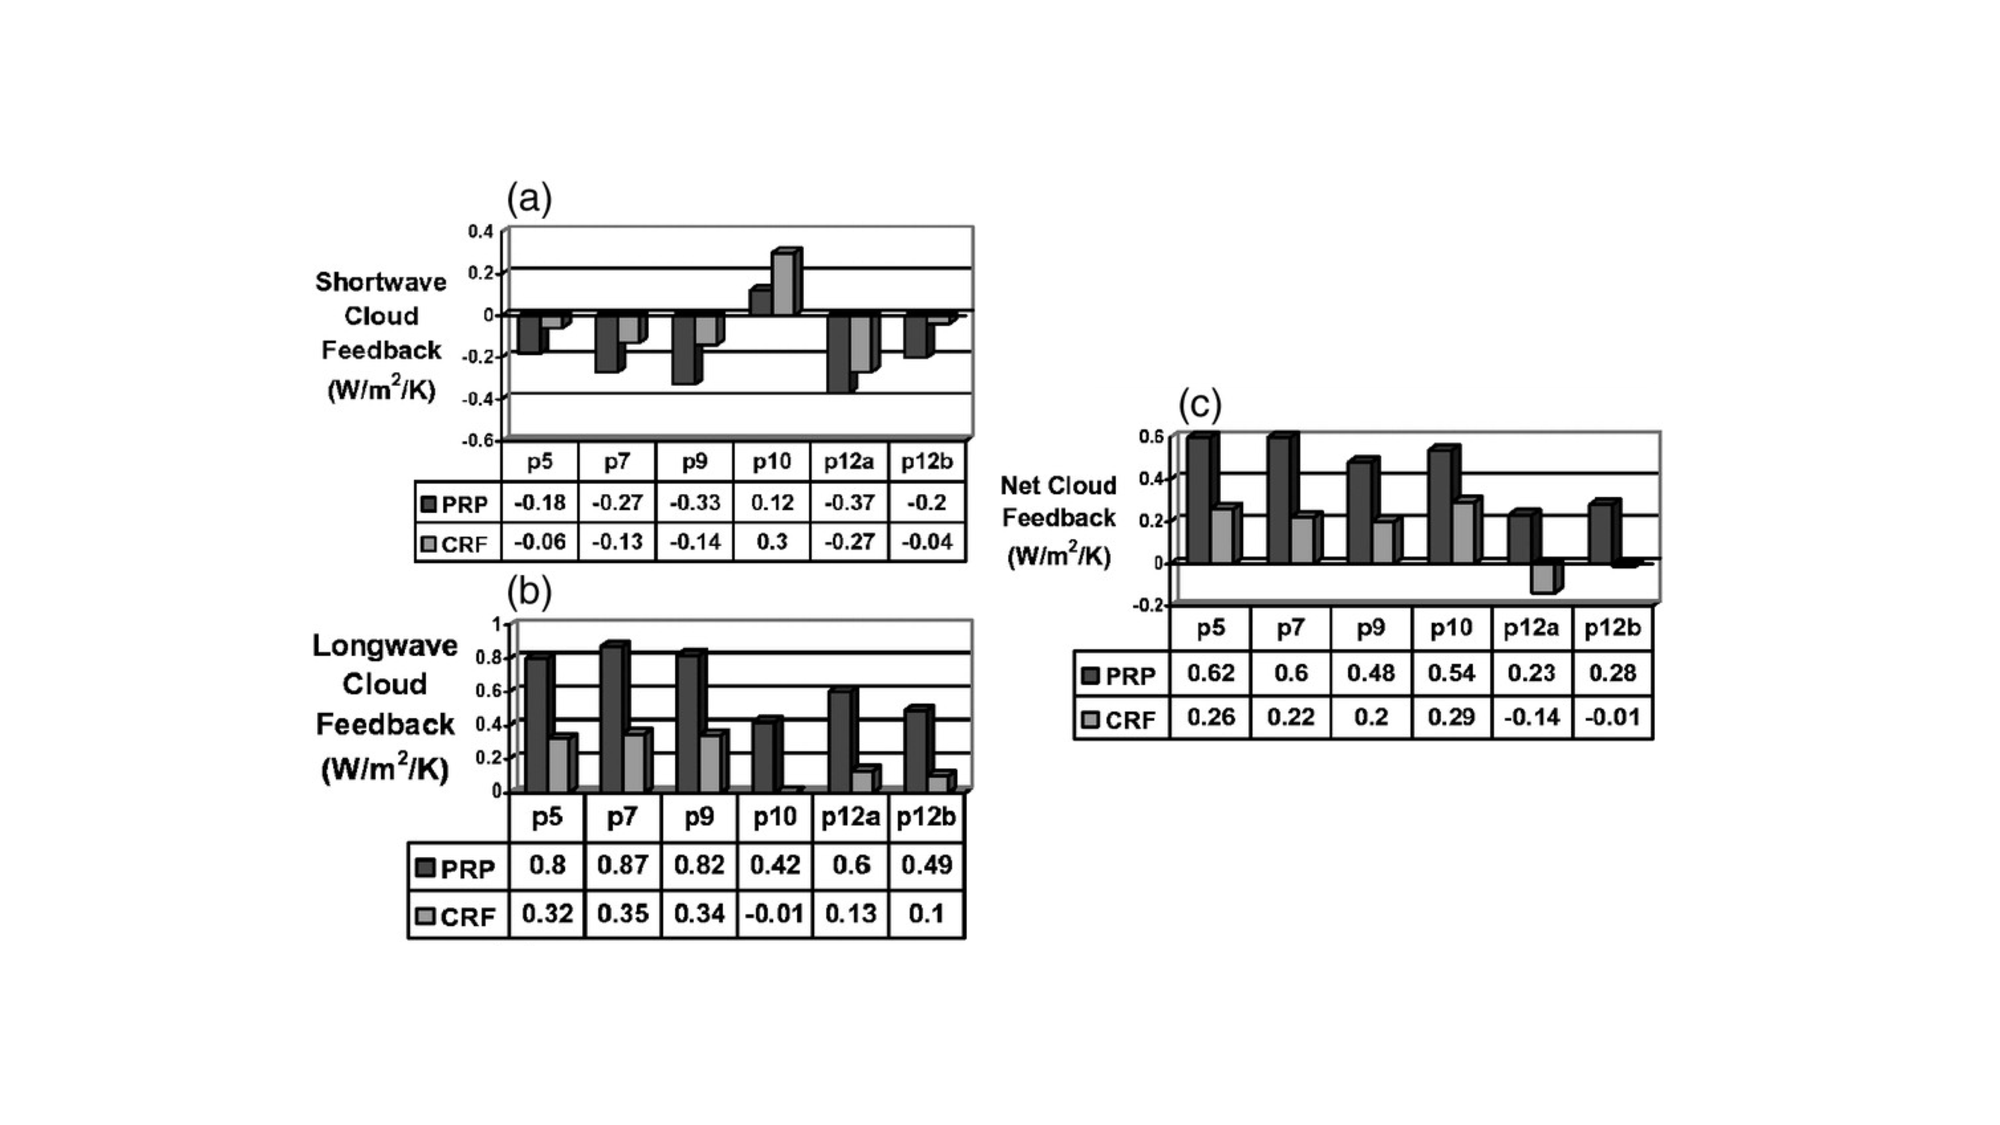
\includegraphics[width=1\linewidth]{{figs/methods/fig2_Soden2004_PRP_CRF_comparison}.pdf}
    \caption{Comparison of the (a) shortwave, (b) longwave, and (c) net cloud feedback parameters from the PRP and $\Delta$CRF (or $\Delta$CRE) methods. Adapted from Fig. 2 of \cite{Soden2004}.}
    \label{fig:cmp_PRP_CRE_Soden}
\end{figure}
If we assume that $\Delta T$, $\Delta w$, and  $\Delta \alpha_s$ are not zero (i.e. $T'\neq T$,  $w'\neq w$, and  $\alpha_s'\neq \alpha_s$), the only way to get $\Delta {CRE}_{net}=0$ would be the changes in total-sky flux (term within first bracket in \eqref{eq:delta_CRE_no_cld_fbk}) and clear-sky flux (term within second bracket in \eqref{eq:delta_CRE_no_cld_fbk}) due to non-cloud feedbacks are equal. However, this is not always the case. An explanation with a simple model is presented in \secref{sec:cld_masking_effect}, but here we provide some simulation results from GCMs first.

Taking the results from \cite{Soden2004} as an example, shortwave (SW), longwave (LW) and net cloud feedback parameters estimated from PRP and $\Delta$CRE mthods from several GFDL AM2 (version numbers denoted as p\#) models are shown in \figref{fig:cmp_PRP_CRE_Soden}. The SW cloud feedback calculated from PRP method is smaller than the ones from $\Delta$CRE method, while the LW cloud feedback from PRP method is larger than that from $\Delta$CRE approach. In total, the magnitude of net cloud feedback from $\Delta$CRE method is underestimated ranges from 0.3 to 0.4 Wm$^{-2}$K$^{-1}$ in AM2 models compared to PRP method. 

\begin{figure}
    \centering
    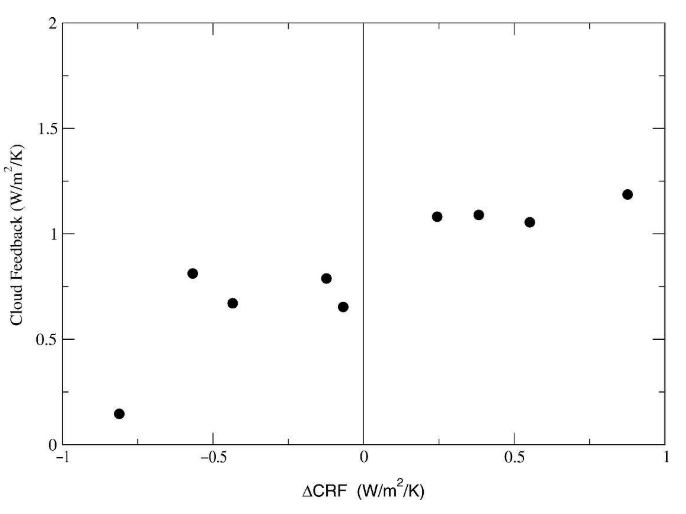
\includegraphics[width=0.65\linewidth]{{figs/methods/Soden_Held_cld_fbk_and_delta_CRF}.png}
    \caption{The cloud feedback parameter plotted as a function of the change in global-mean net cloud radiative forcing per degree change in global surface temperature. Adapted from Fig. 4 of \cite{Soden2006}.}
    \label{fig:cld_fbk_and_CRE_Soden_Held}
\end{figure}

% \begin{figure}
%     \centering
%     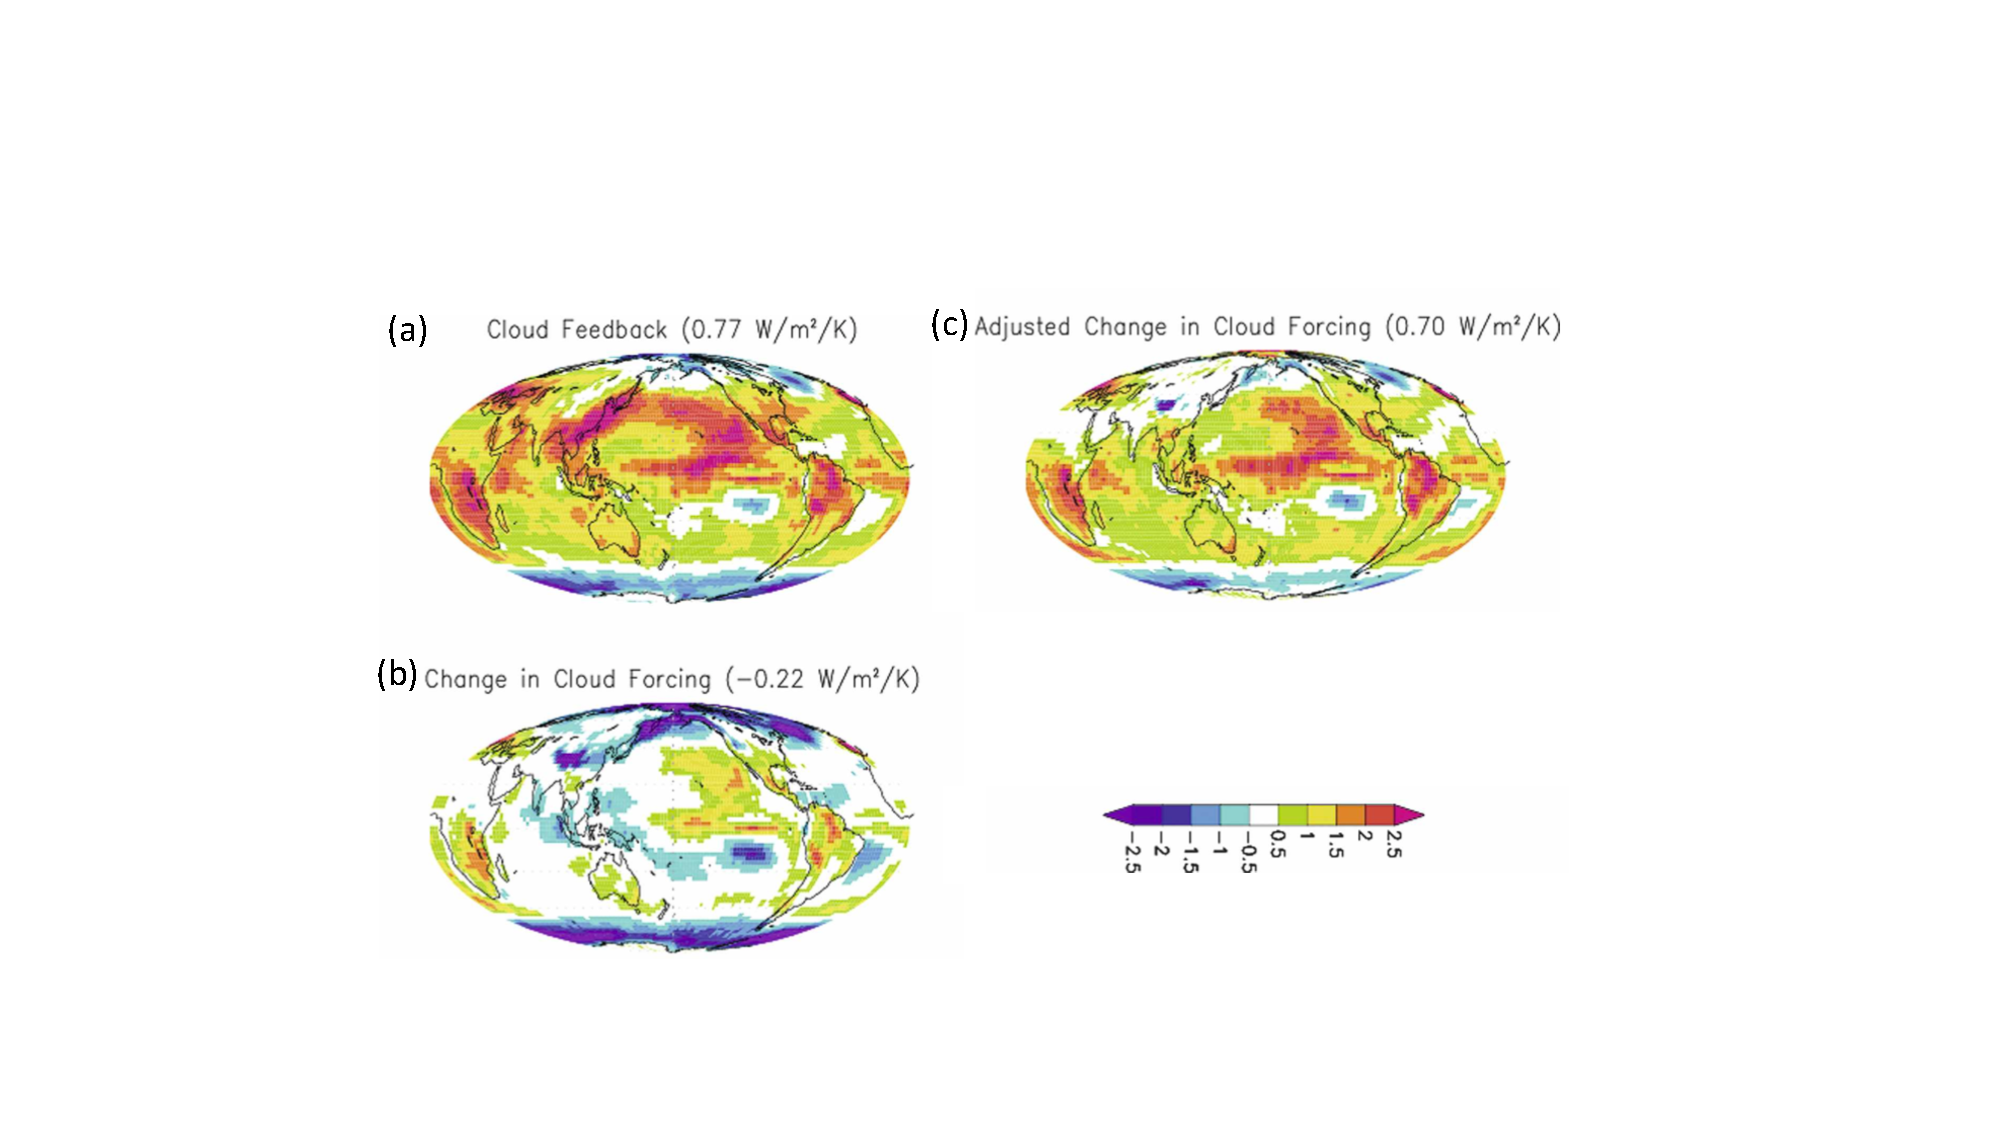
\includegraphics[width=0.9\linewidth]{{figs/methods/cld_fbk_from_kernel_CRF_adjust_forcing}.pdf}
%     \caption{Multimodel ensemble-mean maps of the cloud feedback estimated as (a) the residual of the kernel calculations, (b) the change in cloud forcing, and (c) the change in cloud forcing after adjusting for the effects of cloud masking on noncloud feedbacks and external radiative forcing. Both the cloud feedback and cloud-masking adjustments to the change in cloud forcing are estimated using the GFDL kernel. Adapted from Fig. 11 of \cite{Soden2008}.}
%     %  Only those models for which both the cloud feedback and CRE were available are included in the ensemble mean.
%     \label{fig:cld_fbk_and_CRE_pattern}
% \end{figure}

Similarly, as shown in \figref{fig:cld_fbk_and_CRE_Soden_Held}, \cite{Soden2006} found that all the models from IPCC Fourth Assessment (AR4) have a positive cloud feedback in 21-century climate change experiments, but roughly half the models show a reduction in net CRE (or CRF; and normalized by surface temperature change) in response to climate change. In their study the cloud feedback is estimated by the radiative kernel method. This apparent discrepancy is possibly due to the influence of noncloud feedbacks on the CRE term \citep{Zhang1994,Soden2004}. Therefore, the change of net CRE is not a reliable measure of cloud feedback, as the signs of them are sometimes different (\figref{fig:cmp_PRP_CRE_Soden}c and \figref{fig:cld_fbk_and_CRE_Soden_Held}). However, it is noted that the cloud feedback is correlated with the change in net CRE as displayed in \figref{fig:cld_fbk_and_CRE_Soden_Held}, indicating that intermodel differences in cloud feedback can be estimated by the intermodel differences in the changes of CRE \citep{Soden2006,Bony2006}. %In addition, the spatial patterns of cloud feedback from radiative kernel and $\Delta$CRE approaches are similar, although the magnitude shows large difference (\figsref{fig:cld_fbk_and_CRE_pattern}b and \ref{fig:cld_fbk_and_CRE_pattern}c), implying that the $\Delta$CRE method is still valuable to have a quick look of the cloud feedback pattern.

\subsection{Cloud masking effect}
\label{sec:cld_masking_effect}

A modified simple thought experiment from \cite{Soden2008} is adopted here to explain what cloud masking effect is and why the two right-hand terms in \eqref{eq:delta_CRE_no_cld_fbk} are usually not equal with each other. As illustrated in \figref{fig:cld_masking_effect}, we assume part of the grid is covered by high clouds (cloud fraction is $f$), and the water vapor contents are $q_1$ and $q_2$ for clear and cloudy subgrid regions, respectively. Here we focus on LW radiation only and assume the LW radiation emitted by water vapor is a linear function of its content, that is $\alpha + \beta q$, where $\alpha$ and $\beta$ are assumed linear coefficients and $\beta$ is negative so that the outgoing LW radiation decreases with the increase of water vapor. The outgoing LW radiation emitted from clouds is regarded as a constant $W$.

\begin{figure}
    \centering
    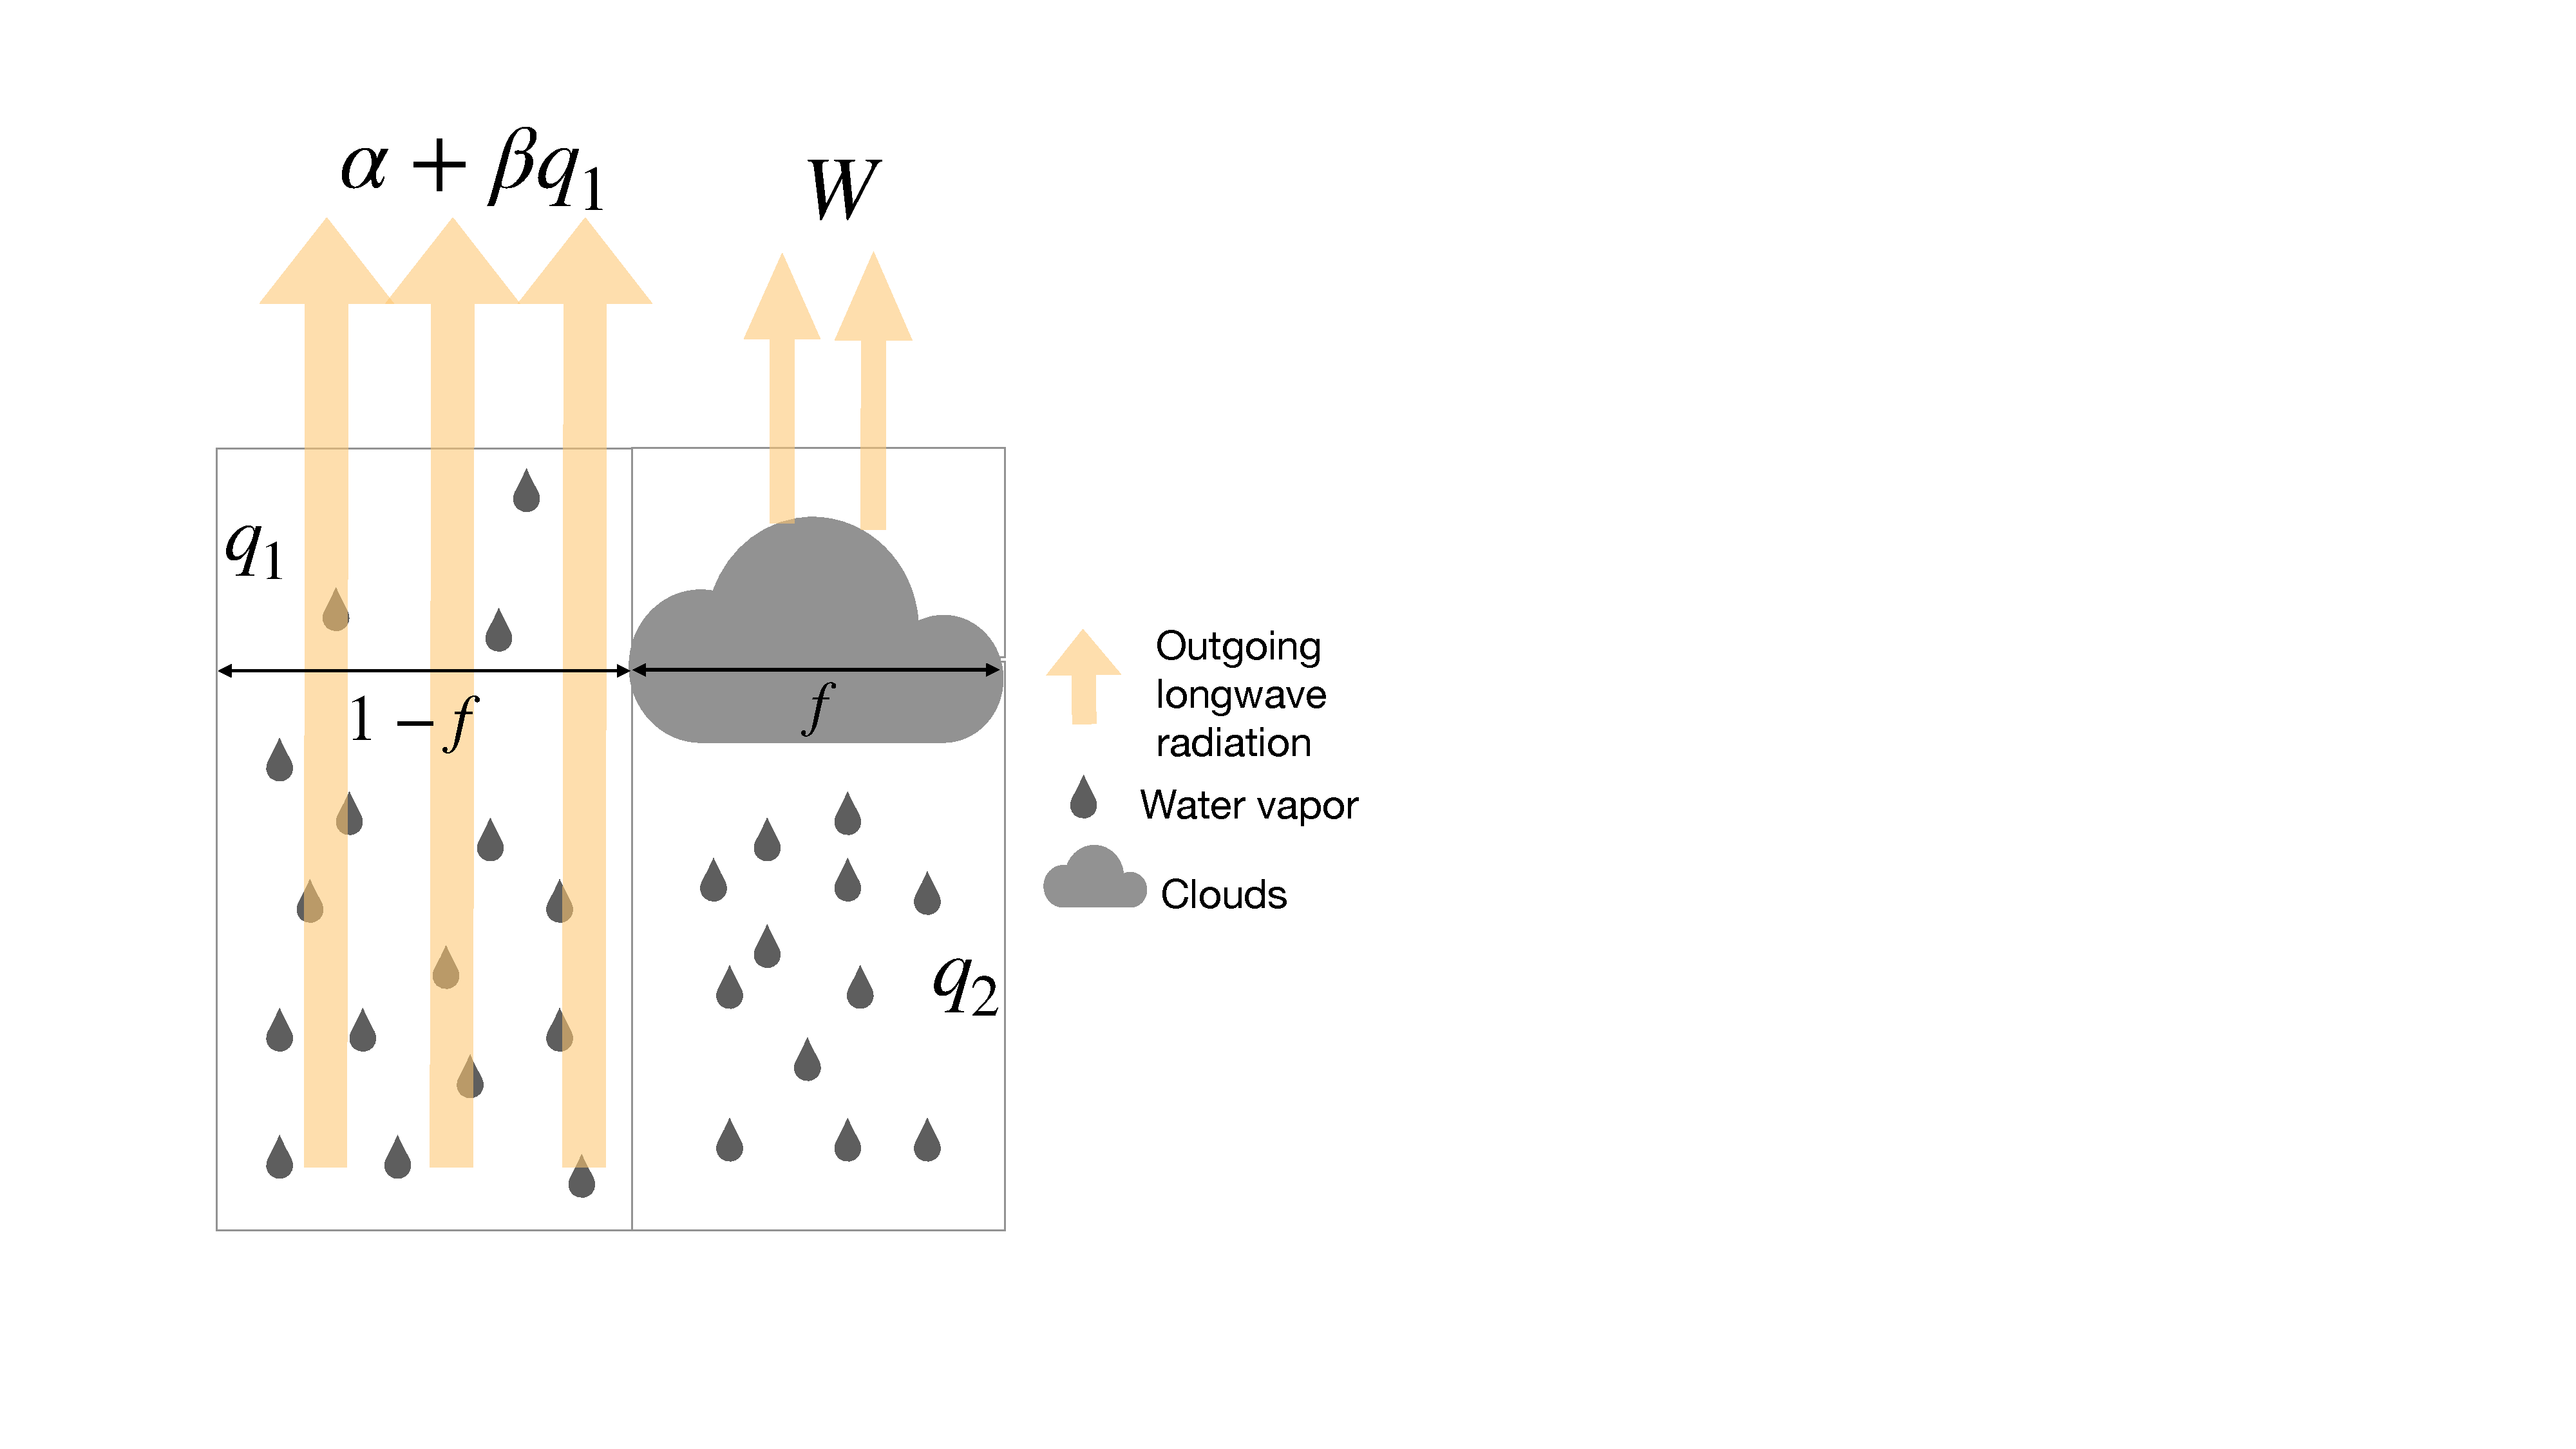
\includegraphics[width=0.65\linewidth]{{figs/methods/cloud_masking_effect}.pdf}
    \caption{Illustration of cloud masking effect on noncloud feedbacks in a grid box.}
    \label{fig:cld_masking_effect}
\end{figure}

If there is no clouds in this grid (i.e. $f=0$), the net LW radiation flux at TOA (downward positive) is $-[\alpha + \beta(q_1+q_2)]$. When clouds are present, the grid averaged net LW flux at TOA becomes
\begin{equation}
    R = - (\alpha + \beta q_1)(1-f)- Wf,
    \label{eq:cld_masking}
\end{equation}
as the LW raditation emitted from water vapor $q_2$ is masked by clouds. Consider a climate change case in which the water vapor and cloud fraction change a bit, and the change in $R$ can be written as follows by differencing \eqref{eq:cld_masking}:
\begin{equation}
    \delta R = \delta R_f + \delta R_q,
\end{equation}
where
\begin{equation}
    \delta R_f = (\alpha + \beta q_1 - W)~\delta f,
    \label{eq:lw_change_due_to_cld}
\end{equation}
and
\begin{equation}
    \delta R_q = -(1-f)\beta~\delta q_1.
    \label{eq:lw_change_due_to_q}
\end{equation}
Now reconsider the situation in \eqref{eq:delta_CRE_no_cld_fbk}, in which there is no cloud feedback ($\delta f=0$), so the LW radiation change at TOA due to clouds is also zero, namely $\delta R_f=0$ in \eqref{eq:lw_change_due_to_cld}. However, as for the  LW radiation flux change due to water vapor perturbation, the cloud fraction $f$ is also included as in \eqref{eq:lw_change_due_to_q}, indicating that clouds have masking effect on the water vapor feedback and the $\delta R_q$ under clear-sky should be different from the one under cloudy condition. 

This simple thought experiment has illustrated that the presence of clouds can have impact on the radiation associated with noncloud variables. That is why the the two right-hand terms in \eqref{eq:delta_CRE_no_cld_fbk} are usually not equal with each other, and it also implies that estimating cloud feedback from changes of cloud radiative effect is probably not a good option due to the cloud masking effect.

\subsection{Cloud radiative kernel method}
\label{sec:Zelinka_method}
In genreal, previous methods introduced in \secref{sec:three_climate_fbk_methods} can give us an estimate of integrated quantity of cloud feedback. Of course, the method such as PRP and radiative kernel can also generate other types of cloud feedbacks by perturbing the corresponding properties, but it is usually hard to do so. To solve this problem, \cite{Zelinka2012computing1,Zelinka2012computing2} propose a new technique based on cloud radiative kernel and the histograms of cloud fraction partitioned by CTP and $\tau$, which can easily attribute the contributions of specific types of cloud changes to cloud feedback.

In this method, the cloud kernel $K$ in each histogram bin of \figref{fig:cld_rad_kernel_Zelinka} is defined as
\begin{equation}
    K = \frac{\partial R}{\partial C},
\end{equation}
which quantifies the sensitivity of TOA radiative flux to cloud fraction changes ($\Delta C$), and is estimated offline from radiation transfer code for each CTP-$\tau$ bin. The process is complicated and detailed description can be found from \cite{Zelinka2012computing1}. The LW, SW and net cloud radiative kernel results are shown in \figref{fig:cld_rad_kernel_Zelinka}, and the major features are:
\begin{enumerate}
    \item The LW cloud radiative kernel is positive for all bins, as the LW CRE is positive. It increases dramatically with cloud top height, and is small near surface as the cloud top temperature contrast with surface is small.
    \item The SW cloud radiative kernel is negative for all bins, as the SW CRE is negative. Its magnitude increases dramatically with optical depth, and almost insensitive to cloud top height.
    \item The net cloud radiative kernels for the lower and thicker clouds are negative, as the SW reflection exceeds LW trapping; while for higher and thinner clouds, the net cloud radiative kenrel are positive, as LW trapping exceeds SW reflection.
\end{enumerate}

\begin{figure}
    \centering
    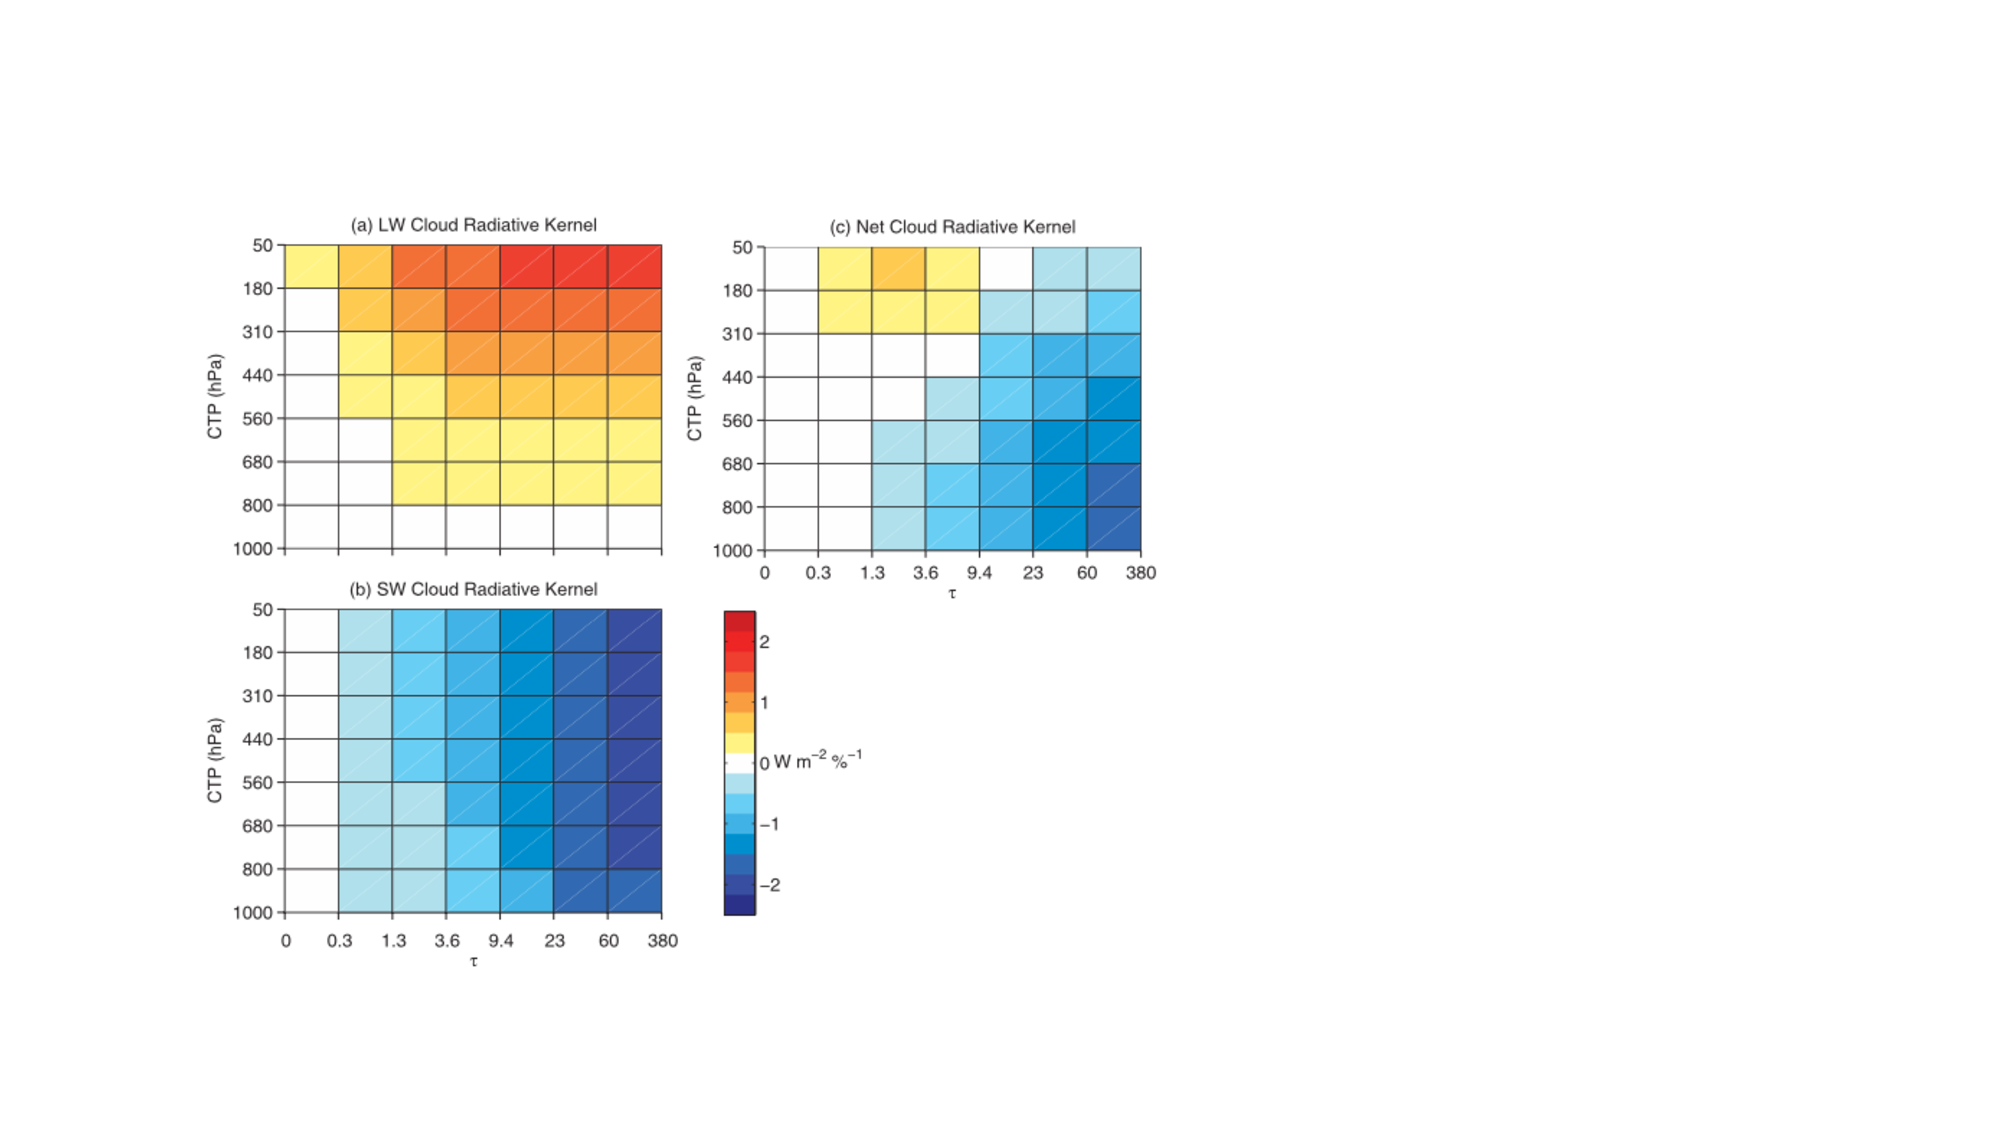
\includegraphics[width=1\linewidth]{{figs/methods/cld_kernel_Zelinka}.pdf}
    \caption{Global, annual, and ensemble mean (a) LW, (b) SW, and (c) net cloud radiative kernels. Adapted from Fig. 1 of \cite{Zelinka2012computing1}}
    % In each model, the kernels have been mapped to the control climate's clear-sky surface albedo distribution before averaging in space; thus, the average kernels are weighted by the actual global distribution of clear-sky surface albedo in each model.
    \label{fig:cld_rad_kernel_Zelinka}
\end{figure}

Multiplying the cloud radiative kernel $K$ by the change in cloud fraction histogram ($\Delta C$, differencing the histogram outputs from cloud simulator) can estimate the contribution of each cloud type to the change in TOA radiation associated with climate change:
\begin{equation}
    \Delta R = K \Delta C
\end{equation}
and hence the cloud feedback is calculated as follows:
\begin{equation}
    \lambda_c = K \frac{\Delta C}{\Delta T_s} = \frac{\Delta R}{\Delta {T}_s}.
\end{equation}
Note that the $\Delta R$ and cloud feedback paramter $\lambda_c$ are function of CTP, $\tau$, latitude, longitude and time, so it can be used to estimate cloud feedback from certain cloud types (according to CTP and $\tau$).


\section{Low cloud amount proxy}

\subsubsection{Low-tropospheric stability}

\cite{Klein1993} studied the seasonal cycle of low stratiform clouds with the data from the Earth Radiation Budget Experiment and found that the low-tropospheric stability (LTS) has a good linear relationship with the low stratus amount, which is applied in Community Atmosphere Model \citep{Collins2004}. In the scheme, LTS can be seen as a measure of the inversion strength and is defined as the potential temperature difference between 700 hPa ($\theta_{700}$) and surface ($\theta_s$),
\begin{equation}
	LTS=\Delta \theta \equiv \theta_{700} - \theta_s.
\end{equation}

\subsubsection{Estimate inversion strength}

\begin{figure}
    \centering
    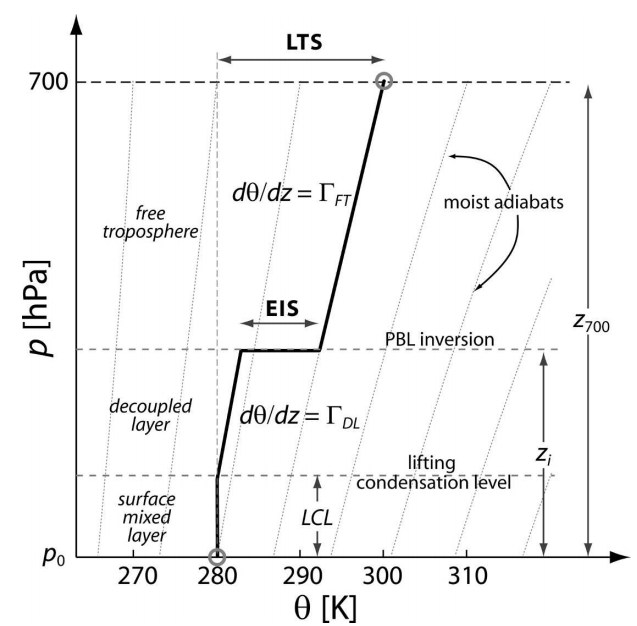
\includegraphics[width=0.8\linewidth]{{figs/methods/Wood_EIS}.png}
    \caption{Idealized profile (thick solid line) of lower-tropospheric structure during periods of undisturbed flow. Moist adiabats are shown as light dotted lines. Adapted from \cite{Wood2006}.}
    \label{fig:wood_eis_atm_profile}
\end{figure}

Despite the widely use of LTS in climate models, \cite{Wood2006} argued that it has yet to be demonstrated
whether the observationally derived LTS-CF relationships will hold in a changed climate. They proposed a new proxy called estimate inversion strength (EIS) to represent the planetary boundary
layer inversion strength and proved that it is better to indicate the low stratiform cloud cover. An idealized profile of lower-tropospheric structure is shown by a thick solid line in Figure \ref{fig:wood_eis_atm_profile}, where the atmospheric conditions roughly follow a dry adiabat below the lifting condensation level (LCL), and then a moist adiabat above. The EIS is defined as
\begin{equation}
    EIS=LTS-\Gamma_{m}^{700} z_{700}+\Gamma_{m}^{LCL} z_{LCL},
    \label{eq:eis}
\end{equation}
or simplified as
\begin{equation}
    EIS=LTS-\Gamma_{m}^{850}\left(z_{700}-z_{LCL}\right),
\end{equation}
where 
\begin{equation}
    \Gamma_{m}(T, p)=\frac{g}{c_{p}}\left[1-\frac{1+L_{v} q_{s}(T, p) / (R_{a} T)}{1+L_{v}^{2} q_{s}(T, p) / (c_{p} R_{v} T^{2})}\right],
    \label{eq:gamma_m}
\end{equation}

\begin{equation}
	z_{700}=\frac{R_{a} T_{0}}{g} \ln \left(\frac{p_{0}}{700~ \mathrm{hPa}}\right).
	\label{eq:z700}
\end{equation}
In \Eqref{eq:eis}, $\Gamma_{m}$ is the moist-adiabatic potential temperature gradient, $z_{700}$ is the height of 700 hPa, $z_{LCL}$ is the height of the lifting condensation level. In \Eqref{eq:gamma_m}, $L_v=2.47\times 10^6$ J kg$^{-1}$ is the latent heat of vaporization. $q_s(T,p)$ is the saturation mixing ratio, and is a function of temperature and pressure derived from the Clausius-Clapeyron equation. $R_a=287.04$ J kg$^{-1}$ K$^{-1}$ and $R_v=461.50$ J kg$^{-1}$ K$^{-1}$ are the gas constants
for dry and water vapor, respectively, $g=9.8$ kg m$^{-2}$ is the gravitational acceleration, and $c_p=1005.0$ J kg$^{-1}$ K$^{-1}$ is the specific heat of air at constant pressure. In \Eqref{eq:z700}, $T_0$ and $p_0$ (in units of hPa) are the surface temperature and pressure respectively.

\subsubsection{Estimated cloud-top entrainment index}

The recent proposed predictors of low cloud amount are also considered in this study: one is the estimated cloud-top entrainment index (ECTEI) by \cite{Kawai2017} and the other is the estimated low-level cloud fraction (ELF) by \cite{Park2019}. 

The ECTEI is a modification of estimated inversion strength (EIS) and takes into account a cloud-top entrainment criterion and is defined as
\begin{equation}
    \mathrm{ECTEI} \equiv \mathrm{EIS} - \beta\left(L_v / c_{p}\right)\left(q_{surf}-q_{700}\right),
    \label{eq:ectei_Kawai}
\end{equation}
where
\begin{equation}
    \beta=(1-k) C_{q\_gap}.
\end{equation}
In \Eqref{eq:ectei_Kawai}, $L_v$ is latent heat of vaporization, and $c_p$ is the specific heat of air at constant pressure. The values of both parameters are the same as the ones in  \Eqref{eq:gamma_m}. $q_{surf}$ and $q_{700}$ are the specific humidity at surface and 700 hPa respectively. The coefficient $C_{q\_gap}$ is the ratio of the total water specific humidity ($q_t$) gap at
the inversion and the $q$ difference between the surface
and 700 hPa. \cite{Kawai2017} estimated the $C_{q\_gap} = 0.76, k=0.70 $ and $\beta = 0.23$ based on radiosonde observation data off the coast of Peru. 
\cite{Park2019} argued that the use of LTS and EIS as a global proxy for low cloud amount is limited
due to their weaker and inconsistent relationship with low cloud amount over land. They kept the calculation of height of inversion, the term with which was neglected in the derivation of EIS \citep{Wood2006}. 